\section{Hyperledger Fabric}\label{sec:hyperledger}

As the popularity of public blockchain and a few other derivative technologies grew, interest in applying the underlying technology of the blockchain, distributed ledger, and distributed application platform to more innovative enterprise use cases also grew. However, many enterprise use cases require performance characteristics that permissionless blockchain technologies are unable (presently) to deliver. In addition, in many use cases, the identity of the participants is a hard requirement, such as in the case of financial transactions where Know-Your-Customer (KYC) and Anti-Money Laundering (AML) regulations must be followed \cite{POLGE2020}.

For enterprise use, it is necessary to consider the following requirements:

\begin{itemize}
\item Participants must be identified/identifiable;
\item Networks need to be permissioned;
\item High transaction throughput performance;
\item Low latency of transaction confirmation;
\item Privacy and confidentiality of transactions and data of business transactions.
\end{itemize}

These requirements are a good fit with the required non-functional requirements for an SCM project and the ones specified in table~\ref{table:rnf}. While many early blockchain platforms are currently being adapted for enterprise use, Hyperledger Fabric has been designed for enterprise use from the outset. 

The Hyperledger Project is a collaborative effort to create an enterprise-grade, open-source distributed ledger framework, and codebase. It aims to advance blockchain technology by identifying and realizing a cross-industry open standard platform for distributed ledgers, transforming how business transactions are conducted globally. Hyperledger was established as a project of the Linux Foundation in early 2016 \cite{cachin2016architecture}.

Hyperledger Fabric implements a distributed ledger platform for running smart contracts, leveraging familiar and proven technologies, with a modular architecture allowing pluggable implementations of various functions. One of the multiple projects currently in incubation under the Hyperledger Project \cite{cachin2016architecture}. Hyperledger Fabric is a widely used permissioned blockchain-primarily in enterprise settings to make transactions between multiple businesses more efficient. This implementation defines assets and the transaction instructions. Members of each permissioned network interact with the ledger using chaincode. The Membership identity service manages IDs and authenticates participants. Also, the Access Control List provides additional layers of permission \cite{blockgeeks2018deeper}.

\begin{figure}[htbp]
\begin{center}
  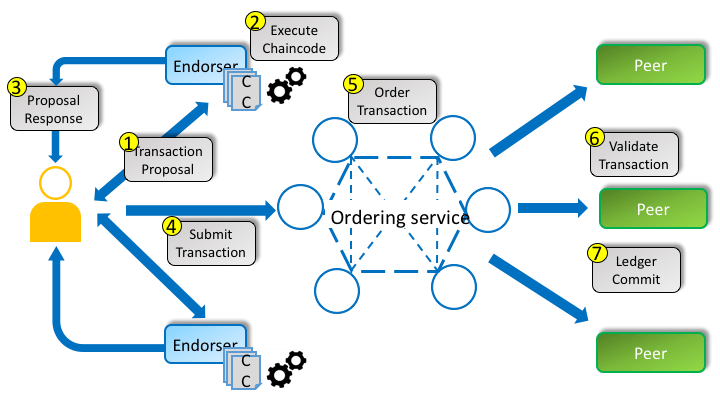
\includegraphics[scale=0.45]{images/Hyperledger-Fabric-high-level-transaction-flow.png}
\caption{Hyperledger Fabric  transaction flow \cite{manevich2018service}.}
\label{fig:hyperledgerFlow}
\end{center}
\end{figure}

There are two types of nodes in Hyperledger Fabric: peer nodes and ordering nodes. Peer nodes are responsible for executing and verifying transactions while ordering nodes are responsible for ordering transactions and propagating the correct history of events to the network. This increases efficiency and scalability by allowing peer nodes to batch and process multiple transactions \cite{buterin2016smart}. 

Fabric Ledger comprises two components: A blockchain log to stores the immutable sequenced record of transactions in blocks and a State Database to maintain the blockchain's current state. In a public blockchain, there is no state database. It means that the chain's current state is always calculated by going through all the transactions in the ledger. For speed and efficiency, the Fabric stores the current state and allows network members to query it as a SQL-like transaction \cite{blockgeeks2016blockchain}. 

Figure~\ref{fig:hyperledgerFlow} shows the Hyperledger Fabric transaction flow. The client (yellow actor) proposes a transaction to the endorsing peers (blue) and collects transaction responses. The client then submits a transaction to the ordering service, which orders incoming transactions and cuts them into blocks. Peers (green) pull blocks from the ordering service, validate the transactions, append them to the ledger, and apply valid transactions to the state.

The log aims to trap an asset providence or place of origin as it exchanges among multiple parties. To track an asset's provenance means to track where and when it was created, and every time it was exchanged. Tracking an asset's providence is extremely important in business because it ensures that the business selling an item possesses a chain of titles verifying their ownership of it. In typical databases, where only the current state is kept and not a log of all transactions, tracking an asset providence becomes very difficult. Add to this the fact that transacting businesses each keep an incomplete record of the asset transaction, and it becomes nearly impossible \cite{blockgeeks2016blockchain}.

Hyperledger fabric uses Private Channels to solve the problem of sensitive information which other parties or competitors could see in a public blockchain. Private Channels are restricted message paths that can provide transaction privacy and confidentiality for a specific subset of network members. All data, including transactions, member, and channel information, are invisible and inaccessible to any network members not explicitly granted access to that channel. This allows competing business interests and any groups that require private, confidential transactions to coexist on the same permissions network \cite{brabbani2017hashing}.
